\documentclass[a4paper,14pt]{extarticle}
\usepackage[utf8]{inputenc}
\usepackage[russian]{babel}
\usepackage{graphicx}
\usepackage[top=0.8in, bottom=0.8in, left=0.8in, right=0.8in]
{geometry}
\usepackage{pgfplots}
\usepackage{amsmath}
\usepackage{setspace}
\usepackage{titlesec}
\usepackage{float}
\usepackage{chngcntr}
\usepackage{pgfplots}
\usepackage{amsfonts}
\usepackage{pgfplotstable}
\usepackage{multirow}
\usepackage{karnaugh-map}
\usepackage{tikz,xcolor}
\usepackage{indentfirst} % Красная строка
\usepackage{listings}
\usepackage{amssymb}
\usepackage{xcolor}
\usepackage{hyperref}

\definecolor{linkcolor}{HTML}{0000FF} % цвет ссылок
\definecolor{urlcolor}{HTML}{FF00FF} % цвет гиперссылок

\hypersetup{pdfstartview=FitH, linkcolor=linkcolor,urlcolor=urlcolor, colorlinks=true}


\titleformat{\section}[hang]
  {\bfseries}
  {}
  {0em}
  {\hspace{-0.4pt}\large \thesection\hspace{0.6em}}
  
  
\titleformat{\subsection}[hang]
  {\bfseries}
  {}
  {0em}
  {\hspace{-0.4pt}\large \thesubsection\hspace{0.6em}}

%\linespread{1.3} % полуторный интервал
%\renewcommand{\rmdefault}{ftm} % Times New Roman

\newcommand{\nx}{\overline{x}}
\newcommand{\p}{0.31}
\newcommand{\scale}{1.4}

\counterwithin{figure}{section}
\counterwithin{equation}{section}
\counterwithin{table}{section}

\begin{document}
\begin{titlepage}
\centering
Санкт-Петербургский политехнический университет Петра Великого \\
\vspace{0.15cm}
Кафедра компьютерных систем и программных технологий \\
\vspace{6.5cm}

{\centering \textbf{Отчёт по лабораторной работе} \\ 
\vspace{0.15cm}
\textbf{Дисциплина}: Телекоммуникационные технологии \\
\vspace{0.15cm}
\textbf{Тема}: Цифровая модуляция.} \\


\vspace{6.5cm}

\begin{table}[H]
\begin{tabular}{p{\textwidth}@{}r}
{Выполнил студент гр. 33501/2} \hfill {Вахаев И.Н.} \\
{Преподаватель} \hfill {Богач Н.В.} \\
\end{tabular}
\end{table}
\vfill

{\centering Санкт-Петербург \\ 
\vspace{0.15cm}
\today}
\end{titlepage}

\tableofcontents

\newpage

\section{Цель работы}

Изучение методов модуляции цифровых сигналов.

\section{Постановка задачи}

\begin{enumerate}
\item Получить сигналы BPSK, PSK, OQPSK, genQAM, MSK, MFSK модуляторов

\item Построить их сигнальные созвездия

\item Провести сравнение изученных методов модуляции цифровых
сигналов

\end{enumerate}

\section{Теоретический раздел}

Модуляция – это процесс изменения каких-либо параметров несущего сигнала под действием информационного потока. Данный термин обычно применяют для аналоговых сигналов. Применительно к цифровым сигналам существует другой термин "манипуляция однако его часто заменяют все тем же словом "модуляция"подразумевая, что речь идет о цифровых сигналах. В цифровой модуляции аналоговый несущий сигнал модулируется цифровым битовым потоком.

Существует 3 основных вида манипуляции сигналов (или шифтинга) и один гибридный:
\begin{enumerate}
\item ASK – Amplitude shift keying (Амплитудная двоичная модуляция).
\item FSK – Frequency shift keying (Частотая двоичная модуляция).
\item PSK – Phase shift keying (Фазовая двоичная модуляция).
\item ASK/PSK.
\end{enumerate}
Этот набор манипуляций определяется основными характеристиками, которыми обладает любой сигнал.

\subsection{Амплитудная модуляция}
При амплитудной манипуляции каждому цифровому символу сопоставляется своя амплитуда несущего
сигнала. Частота и фаза манипулированного сигнала остаются неизменными. Амплитудная манипуляция
редко используется на практике, т.к. из всех видов манипуляции наименее помехоустойчива. Амплитудная
манипуляция обычно применяется в сочетании с другими видами манипуляции.

\subsection{Частотная модуляция}

При частотной манипуляции каждому цифровому символу сопоставляется своя частота несущего сигнала.
Амплитуда и фаза манипулированного сигнала не меняются. Частотно-манипулированные FSK сигналы
одни из самых распространенных в современной цифровой связи. Это обусловлено прежде всего простотой их генерирования и приема, ввиду нечувствительности к начальной фазе.

\subsection{Фазовая модуляция}
При фазовой манипуляции каждому цифровому символу сопоставляется своя начальная фаза несущего сигнала при неизменной амплитуде. Данный вид манипуляции наиболее сложен в реализации, но и наиболее помехоустойчив по сравнению с двумя другими видами манипуляции.
В настоящее время разработано несколько вариантов двухпозиционной (бинарной) и многопозиционной фазовой манипуляции. В радиосистемах передачи информации наиболее часто применяются двоичная, четырех позиционная и восьми позиционная фазовая манипуляция (ФМн). Данные сигналы обеспечивают
высокую скорость передачи, применяются в радиосвязи, в системах фазовой телеграфии, при формировании сложных сигналов.
Наиболее простой является бинарная ФМн, при которой изменение фазы несущего колебания происходит скачком в определенные моменты первичного сигнала на 0 или 180o; при этом его амплитуда и частота несущей остаются неизменными.

\subsection{Квадратурная модуляция}

Смысл квадратурно модуляции заключается в представлении гармонического колебания с произвольной фазой линейной комбинацией синусоидального и косинусоидального колебания. Квадратурное представление сигнала заключается в выражении колебания линейной комбинацией двух ортогональных составляющих – квадратурной и синфазной.
Таким образом, в качестве манипулирующих сигналов используют сигналы, отличающиеся по структуре от исходных передаваемых двоичных сигналов, для формирования которых используется специальное кодирующее устройство - кодер модулятора.

\section{Ход работы}

\subsection{BPSK}


\begin{figure}[H]
\center{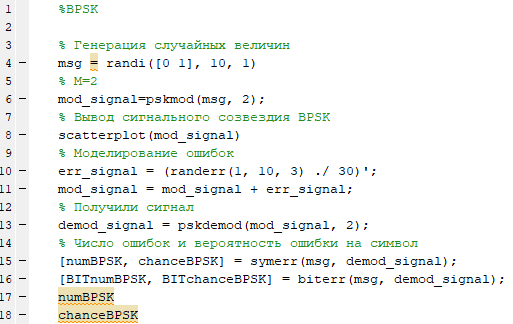
\includegraphics[width=1\linewidth]{screen/1}}
\caption{Код BPSK в Matlab}
\label{1}
\end{figure}

\begin{figure}[H]
\center{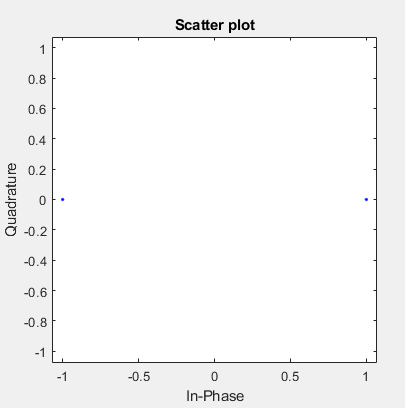
\includegraphics[width=1\linewidth]{screen/2}}
\caption{Сигнальное созвездие BPSK}
\label{2}
\end{figure}


\subsection{PSK}

\begin{figure}[H]
\center{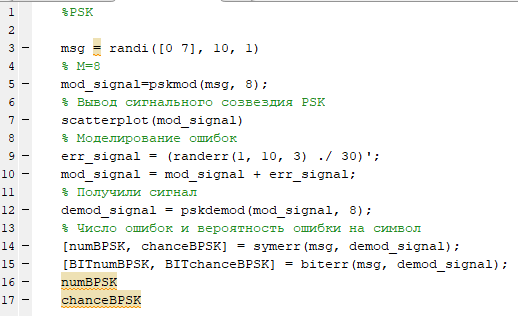
\includegraphics[width=1\linewidth]{screen/3}}
\caption{Код PSK в Matlab}
\label{3}
\end{figure}

\begin{figure}[H]
\center{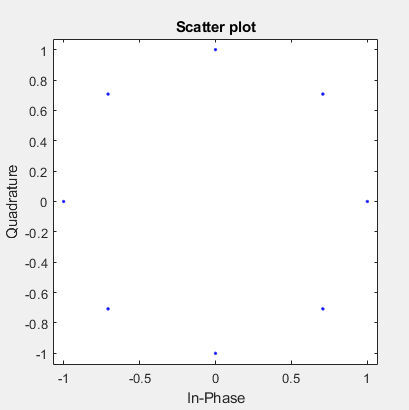
\includegraphics[width=1\linewidth]{screen/4}}
\caption{Сигнальное созвездие PSK}
\label{4}
\end{figure}

\subsection{OQPSK}

\begin{figure}[H]
\center{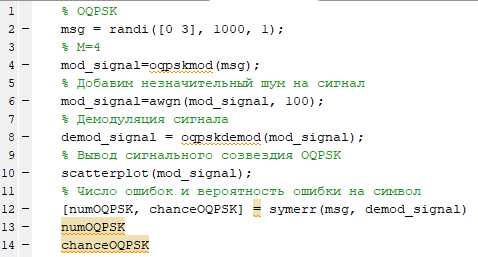
\includegraphics[width=1\linewidth]{screen/5}}
\caption{Код OQPSK в Matlab}
\label{5}
\end{figure}

\begin{figure}[H]
\center{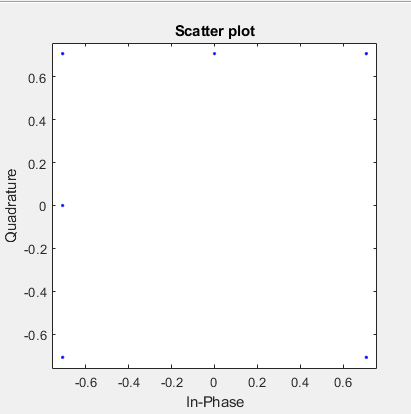
\includegraphics[width=1\linewidth]{screen/6}}
\caption{Сигнальное созвездие OQPSK}
\label{6}
\end{figure}

\subsection{genQAM}

\begin{figure}[H]
\center{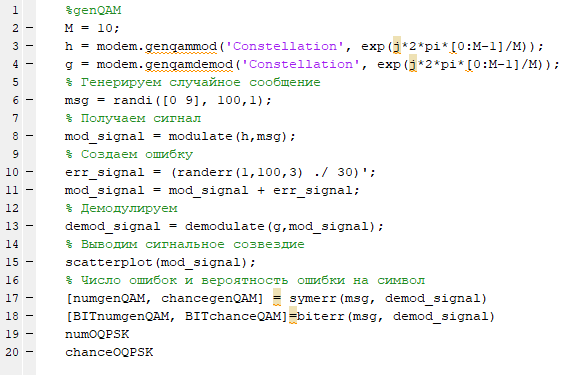
\includegraphics[width=1\linewidth]{screen/7}}
\caption{Код genQAM в Matlab}
\label{7}
\end{figure}

\begin{figure}[H]
\center{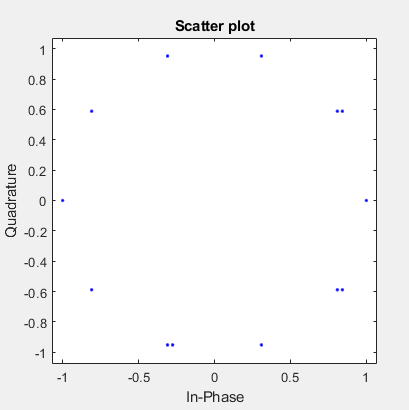
\includegraphics[width=1\linewidth]{screen/8}}
\caption{Сигнальное созвездие genQAM}
\label{8}
\end{figure}


\subsection{MSK}

\begin{figure}[H]
\center{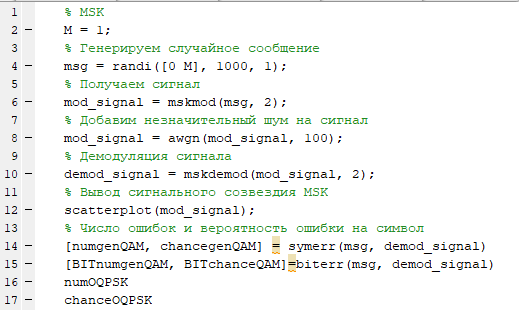
\includegraphics[width=1\linewidth]{screen/9}}
\caption{Код MSK в Matlab}
\label{9}
\end{figure}

\begin{figure}[H]
\center{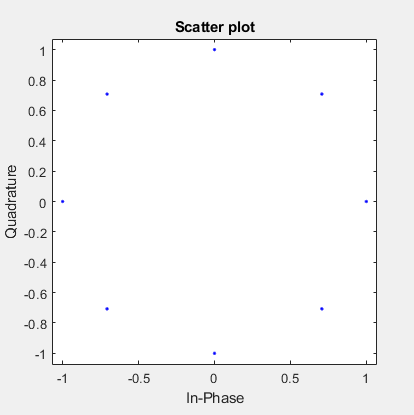
\includegraphics[width=1\linewidth]{screen/10}}
\caption{Сигнальное созвездие MSK}
\label{10}
\end{figure}

\subsection{FSK}

\begin{figure}[H]
\center{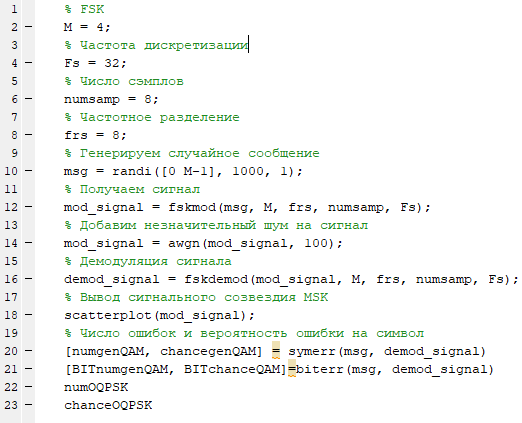
\includegraphics[width=1\linewidth]{screen/11}}
\caption{Код FSK в Matlab}
\label{11}
\end{figure}

\begin{figure}[H]
\center{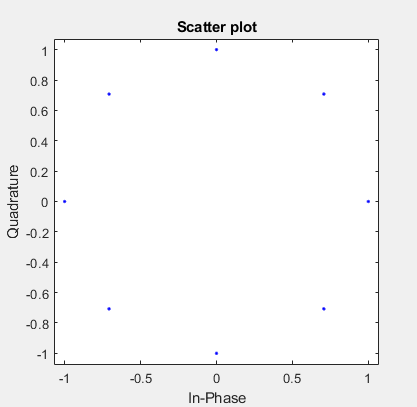
\includegraphics[width=1\linewidth]{screen/12}}
\caption{Сигнальное созвездие FSK}
\label{12}
\end{figure}


\section{Выводы}
Цифровая модуляция - это процесс преобразования цифровых символов в сигналы, совместимые с характеристиками канала. При низкочастотной модуляции эти сигналы обычно имеют вид импульсов заданной формы. В случае полосовой модуляции импульсы заданной формы модулируют синусоиду, называемую несущей волной, или просто несущей; для радиопередачи на нужное расстояние несущая преобразуется в электромагнитное поле.

В данной лабораторной работе были рассмотрены различные виды цифровой модуляции. Тип цифровой модуляции выбирается в зависимости от требований к скорости передачи и помехозащищенности. Самой надёжной считается квадратурная манипуляция, так как информацию можно подавать сразу по двум параметрам. Для повышения скорости передачи могут быть использованы PSK или QAM с большим количеством точек, что в свою очередь негативно скажется на помехоустойчивости вследствие их близкого расположения друг относительно друга на сигнальном созвездии.
Число бит, передаваемых одним состоянием, определяется как Log2N, где N — уровень модуляции. Таким образом, чем выше уровень модуляции, тем больше данных мы можем передать (или потерять) за единицу времени. 



\end{document}